% ============================================================
\begin{figure}[t]
\centering
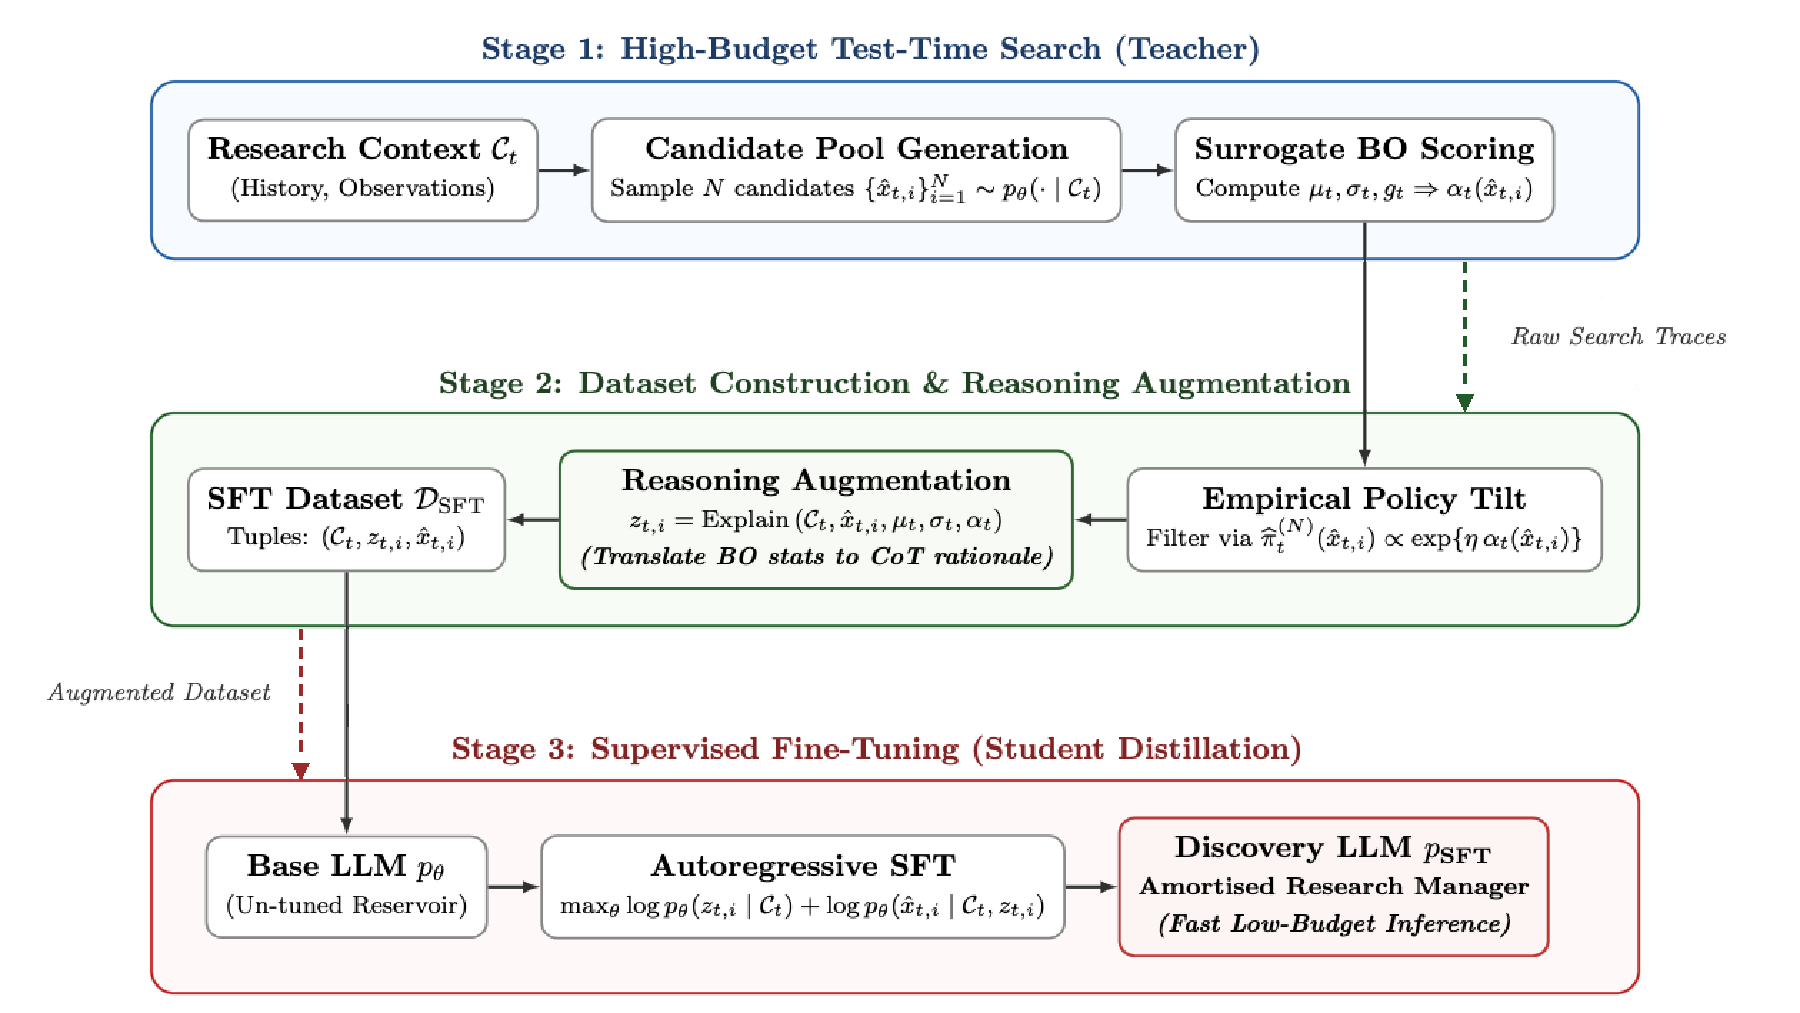
\includegraphics[width=1\textwidth]{figure/workflow.pdf}
\caption{\textbf{Overview of the LDM training pipeline workflow.}
\textbf{Stage 1:} High-budget test-time search generates candidate pools scored
by surrogate acquisition values ($\alpha_t$). \textbf{Stage 2:} High-value
candidates are filtered via an empirical policy tilt $\widehat{\pi}_t^{(N)}$,
and numerical BO statistics are translated into semantic reasoning rationales
($z_{t,i}$) via reasoning augmentation. \textbf{Stage 3:} The base model is
fine-tuned on the CoT target $(z_{t,i}, \hat{x}_{t,i})$ using standard
next-token prediction, compiling the high-budget search policy into an
amortised student model ($p_{\text{SFT}}$) capable of fast, low-budget
inference.}
\label{fig:app-training-pipeline}
\end{figure}

\section{Additional Fine-Tuning Analyses}
\label{app:finetuning-details}
% ============================================================

Section~4.4 describes how high-budget LDM test-time search is distilled into a
student proposer, and Section~6.4 reports the main fine-tuning results on
AutoResearch, antibody design, and small-molecule discovery. This appendix
provides complementary evidence that is not repeated in the main text.

\subsection{Fine-Tuning as Value Distillation}
\label{app:finetune-values}

Modern LLM fine-tuning paradigms can be distinguished by the
decision-theoretic value they distill into the model weights. Chat LLMs distill
human preference value, reasoning LLMs distill verification value, and
Discovery LLMs distill epistemic acquisition value. The object distilled by
LDM is therefore not the measured reward $R(x)$ alone, nor the static
memorisation of a high-reward molecule, protein, or program. Instead, the goal
is to distill the acquisition strategy that decides which scarce experiment is
worth running under uncertainty. Figure~\ref{fig:app-training-pipeline} summarises this three-stage training pipeline: high-budget test-time search, reasoning-augmented dataset construction, and supervised distillation into the student proposer.


Table~\ref{tab:reasoning-augmentation} illustrates how numerical acquisition
evidence is translated into semantic supervision across the three discovery
domains.

\begin{table}[H]
\centering
\small
\begin{tabular}{@{}p{0.18\linewidth}p{0.36\linewidth}p{0.40\linewidth}@{}}
\toprule
\textbf{Domain} & \textbf{Acquisition evidence (Numerical)} & \textbf{Example augmented rationale (Semantic)} \\
\midrule
\texttt{autoresearch} code search &
Best run \texttt{state\_0019} reaches \texttt{val\_bpb} $0.9811$ by lowering \texttt{TOTAL\_BATCH\_SIZE} and tuning \texttt{ASPECT\_RATIO}; several near-best runs also lower the batch size. The current parent already sits at the minimum batch size with only $5$ active parameters and no improvement over the last $4$ rounds. &
Lowering the total batch size has been a robust positive move---more steps fit inside the fixed $30$\,s budget---but that lever is now exhausted and the active parameters have \textbf{plateaued over the last four rounds}, so the set is near its ceiling. Rather than re-tuning saturated knobs, I should \textbf{activate a currently-inactive parameter} (e.g.\ \texttt{MATRIX\_LR}) to open a new optimisation dimension. \\
\addlinespace
Antibody CDRH3 design &
Best sequence \texttt{ADGHTKQNPRW} at $-64.28$; the last four candidates share the fixed prefix \texttt{ADGHTKQNPR} and scan only the final position (W $-64.28$, Y $-62.69$, A $-59.38$, S $-57.96$). &
The history is a single-point scan of the last residue on an already-refined scaffold, with the bulky aromatic W best so far. The informative move is to keep the refined prefix and test an \textbf{untested residue of similar hydrophobic character}---leucine (L)---which may reproduce W's favourable hydrophobic contact; propose \texttt{ADGHTKQNPRL}. \\
\addlinespace
Small-molecule discovery &
$29$ molecules evaluated and the loop is flagged \texttt{stalled}; the top actives ($\sim\!8.1$) share one isoxazolone/thiazolone fused core with isopropoxy and cyano groups, docking $\sim\!-8$. &
Because the loop is stalled and near-duplicates are disallowed, adding a methyl to a known winner carries no information. The higher-value move is a \textbf{recombination or scaffold hop}---e.g.\ combining the pyridine-ring variant with the morpholine side chain into a molecule not yet seen---so the candidate probes a genuinely new region of the Pareto frontier rather than exploiting a saturated one. \\
\bottomrule
\end{tabular}
\vspace{0.5em}
\caption{\textbf{Reasoning augmentation turns numerical acquisition labels into semantic training signals.}
The rationales are faithful (translated and condensed) excerpts of reasoning traces generated by the self-hosted DeepSeek V4 Flash teacher inside the high-budget LDM-TTS loop, one per domain. They describe the epistemic value of managing research progress by reading the evaluated history, diagnosing stagnation, and choosing an information-adding move, rather than focusing only on the domain-specific final solution.}
\label{tab:reasoning-augmentation}
\end{table}

\subsection{Cross-Molecule Transfer without Reasoning Augmentation}
\label{app:finetune-no-augmentation}

We test the minimal form of discovery fine-tuning without an explicit
reasoning target. Training data are collected from high-budget LDM-TTS traces
on a source molecular optimisation task. The Qwen3.5-9B proposer is fine-tuned
on acquisition-weighted examples and then evaluated on a different molecular
optimisation task within the same acquisition-guided LDM loop.

This ablation retains the same LDM state and action schema as the
reasoning-augmented setting, but omits the explicit research-progress
rationale $z_{t,i}$.

This setting shows positive transfer across molecular tasks. The base
Qwen3.5-9B LDM reaches a final hypervolume of $16.489\pm5.867$, whereas the
fine-tuned model reaches $22.279\pm3.828$ under the same evaluation protocol.
Because the discovery data are collected from one molecule and evaluated on
another, the improvement cannot be explained by memorising the final molecules
from the source task. It instead shows that acquisition-weighted fine-tuning
can transfer part of the research-management policy even without an explicit
reasoning channel.

\subsection{Supplementary Quantitative Tables}
\label{app:finetune-tables}

Table~\ref{tab:app-smallmol-cot} retains the G12C results not shown in the
main-text KRAS G12D learning curve. Table~\ref{tab:app-finetune-cot-ablation}
collects the numerical cross-domain comparison underlying the three main-text
figures.

\begin{table}[H]
\centering
\small
\begin{tabular}{@{}lcc@{}}
\toprule
\textbf{Inference policy} & \textbf{KRAS G12C} & \textbf{KRAS G12D} \\
 & HV $\uparrow$ & HV $\uparrow$ \\
\midrule
Qwen3.5-9B base (without\_cot) & $11.64\pm2.63$ & $16.49\pm5.87$ \\
Fine-tuned Qwen3.5-9B (without\_cot) & $14.73\pm3.09$ & $22.28\pm3.83$ \\
DeepSeek V4 Flash (without\_cot) & $18.97\pm1.76$ & $24.55\pm3.59$ \\
DeepSeek V4 Flash (with\_cot) & $19.98\pm2.00$ & $24.07\pm3.12$ \\
\textbf{Fine-tuned Qwen3.5-9B (with\_cot)} & $\mathbf{20.98\pm2.92}$ & $\mathbf{26.66\pm2.61}$ \\
\bottomrule
\end{tabular}
\caption{\textbf{Reasoning-augmentation ablation on small-molecule discovery.}
Final Pareto-front hypervolume at an evaluation budget of 80, averaged over five seeds.}
\label{tab:app-smallmol-cot}
\end{table}

\begin{table}[H]
\centering
\setlength{\tabcolsep}{4pt}
\scriptsize
\begin{tabular}{@{}lcccc@{}}
\toprule
\textbf{Model} & \textbf{CoT} & \textbf{AutoResearch} & \textbf{Antibody} & \textbf{SmallMol} \\
 & & val\_bpb $\downarrow$ & $-E_{\mathrm{bind}}$ $\uparrow$ & HV $\uparrow$ \\
\midrule
Base Qwen3.5-9B & off & $0.9965$ & $102.6$ & $16.49$ \\
Base Qwen3.5-9B & on  & $0.9825$ & $104.4$ & --- \\
LDM-SFT & off & $0.9829$ & $105.1$ & $22.28$ \\
\textbf{LDM-SFT} & \textbf{on} & $\mathbf{0.9788}$ & $\mathbf{105.5}$ & $\mathbf{26.66}$ \\
\midrule
\multicolumn{2}{@{}l}{Qwen3-Coder-30B ref.} & $0.9801$ & --- & --- \\
\bottomrule
\end{tabular}
\caption{\textbf{Cross-domain reasoning-augmentation ablation.}
Terminal metrics for the three fine-tuning studies.}
\label{tab:app-finetune-cot-ablation}
\end{table}

\subsection{In-Distribution Single-Task Fit}
\label{app:finetune-indistribution}

Before evaluating the distilled policies in the acquisition loop, we verify
that each single-task model fits its reasoning-augmented training data. We
track training and held-out losses for \texttt{autoresearch} program search,
small-molecule KRAS design, and antibody CDRH3 design. All three losses
converge within a few dozen steps, while the held-out curves closely track the
training curves. The absolute held-out losses differ by domain: $0.06$ for
\texttt{autoresearch}, $0.38$ for small-molecule design, and $0.70$ for
antibody CDRH3 design. These differences reflect the different action spaces
and target lengths, rather than a failure to fit the data.

\begin{figure}[H]
\centering
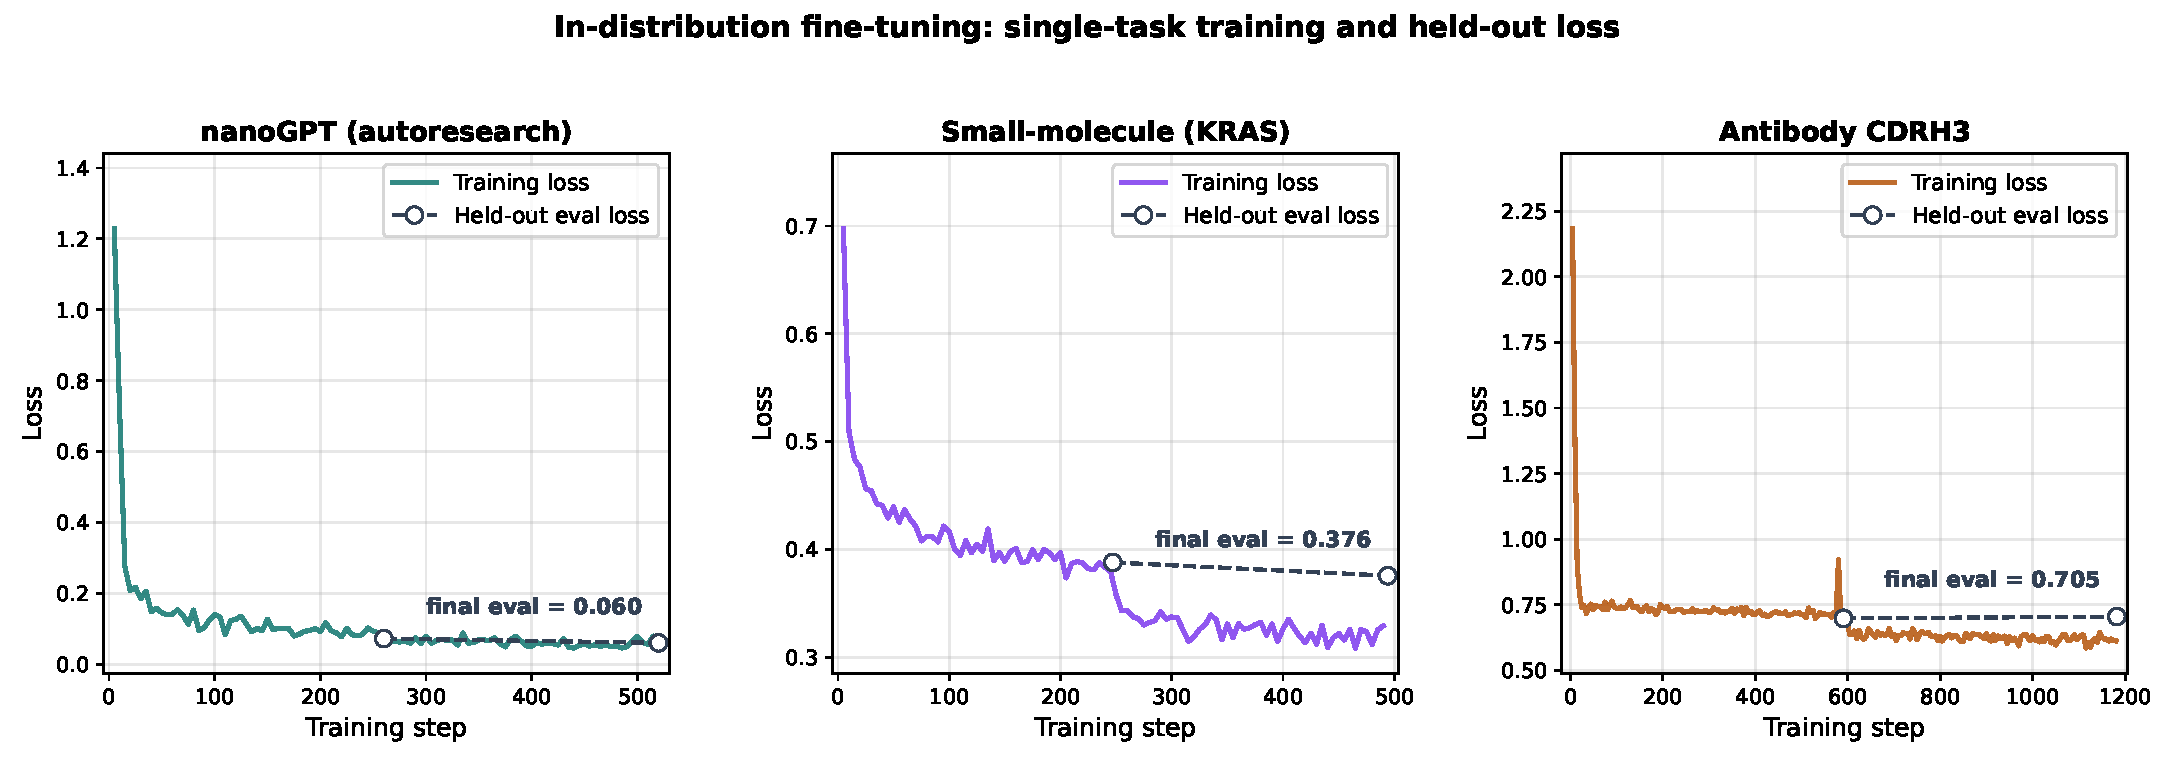
\includegraphics[width=0.95\linewidth]{figure/indist_curves.pdf}
\caption{\textbf{In-distribution single-task fine-tuning.} Training loss
(solid) and held-out evaluation loss (markers) versus training step for the
\texttt{autoresearch}, small-molecule, and antibody CDRH3 policies. All three
converge within a few dozen steps, and the held-out loss tracks the training
loss, confirming a faithful in-distribution fit before acquisition-loop
evaluation.}
\label{fig:app-indist-curves}
\end{figure}

\subsection{Out-of-distribution generalisation to held-out antigens}
\label{sec:finetune-ood}

To test whether it learns
a \text{transferable} acquisition policy rather than memorising antigen-specific patterns, we hold two of the
five antibody targets (\texttt{1FBI\_X}, \texttt{1H0D\_C}) out of training entirely, fine-tune the mixed-task
model on the other three, and evaluate on the held-out pair inside the same acquisition-guided loop, antigens
whose sequences and binding landscapes were never seen during training.

Figure~\ref{fig:protein-ood-mixed32} shows the out-of-distribution model matches or exceeds the
\emph{in-distribution} model (which \emph{was} trained on these antigens) on both held-out targets, and clearly
beats base Qwen3.5-9B with and without chain-of-thought: it reaches $-110.57$ on \texttt{1FBI\_X}
(base $-109.5$, in-distribution $-113.4$) and $-95.4$ on \texttt{1H0D\_C}, where it even surpasses the
in-distribution model ($-94.6$) and the base ($-90.9$). Since the model never observed these antigens, the gain
cannot be memorisation---the distilled acquisition policy transfers to unseen targets. 

\begin{figure}[H]
\centering
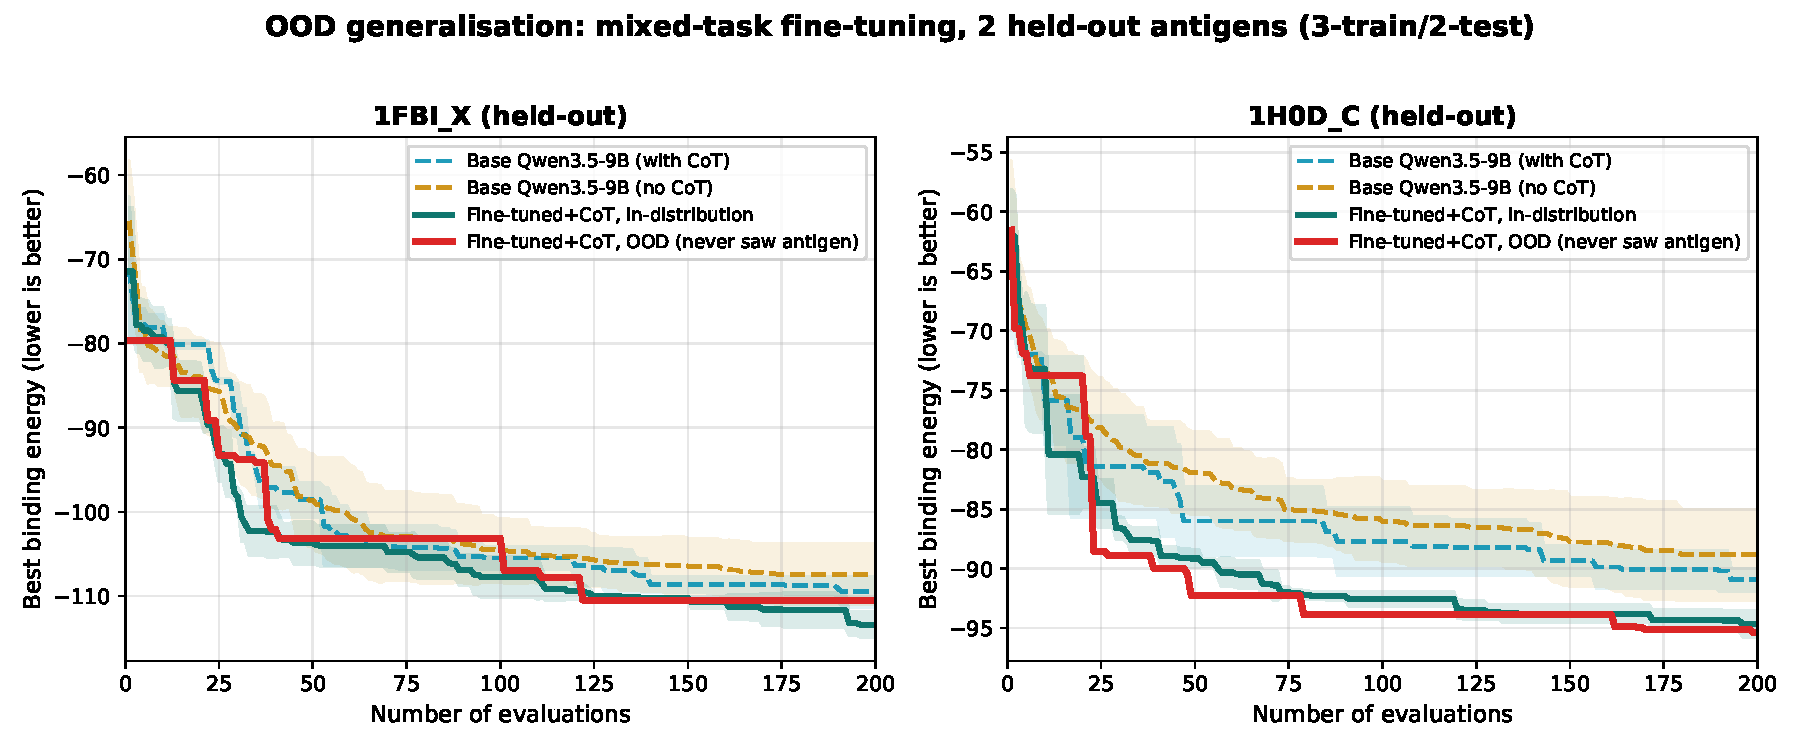
\includegraphics[width=0.98\linewidth]{figure/ood_mixed32.pdf}
\caption{\textbf{Out-of-distribution generalisation to held-out antigens (3-train/2-test).} Best Absolut binding
energy versus number of evaluations on the two held-out antigens. The mixed-task fine-tuned model evaluated on
antigens it never saw during training (red) matches or exceeds the in-distribution fine-tuned model (teal) and
clearly beats base Qwen3.5-9B with and without chain-of-thought (dashed).}
\label{fig:protein-ood-mixed32}
\end{figure}
